%!TEX TS-program = pdflatex
%!TEX encoding = UTF-8 Unicode

\documentclass{unipd-thesis-modern} % src: https://github.com/baronefr/unipd-thesis-modern
%  print layout: two-sided with binding on the left


% I recommend to validate/convert the PDF/A file with the following tool:
% https://www.pdfforge.org/online/en/validate-pdfa


% additional packages
\usepackage{lipsum} % for DEMO only

%% (optional) to add a draft watermark, uncomment the following:
%\usepackage[color={[gray]{0.85}}]{draftwatermark}
%% NOTE: high values -> less visible

% ToC customization
\setlength{\cftbeforechapskip}{7pt} % there are more variables like this set in the template file
\setcounter{tocdepth}{4} % ToC depth


% titles
\title{A modern template for a thesis at\\ the University of Padova}
\thesisHeader{Department of Physics and Astronomy ``G. Galilei''\\PhD Thesis in Physics}
\academicYear{2026/2027}

% student
\author{Student Name Surname}
\studentId{1234567}

% supervisor(s)Zürich
\advisor{Prof. Manuel Rolo}{INFN Turin} % (mandatory)
\coadvisor{Dr. Alberto Tibaldi}{Politechnico di Torino} % (optional, comment to remove)
\otheradvisor{Prof. Paolino Paperino}{University of Padova} % (optional, comment to remove)
% ^ NOTE: you can use optional arg to customize the label "Internal Supervisor"
%   example:   \otheradvisor[The best supervisor!]{Prof. Paolino Paperino}{University of Padua}




% add notes at the bottom of the second page (optional)
\secondpage{\mbox{}
\vfill

{\small\onehalfspacing
\begin{center}

\noindent\rule{\textwidth}{1pt} % ----------

    \LaTeX~document compiled on \today.

\noindent\rule{\textwidth}{.2pt} % ----------

    \textbf{Additional resources}
    
    This template allows you to put some text in the second cover page.\\ 
    The text can be modified in \textit{docs/secondcover.tex}.\\
    I suggest you take this space to refer to any software repository linked to your work,\\ such as the following:\\

    \prettygitlink{sami12398987/Unipd-thesis-template}
\end{center}
} % ----------}

% dedication (comment line to remove)
\dedication{\textit{To my parents\\and friends}}


% define custom symbols and shortcuts (optional)
%!TEX root = ./main.tex

% please use this file to define custom symbols and commands

\newtheorem{prop}{Proposition}
\newtheorem{theorem}{Theorem}

\newcommand{\myvec}[1]{\underline{#1}}

\newcommand{\hamCD}{\mathcal{H}_{\mathrm{CD}}}
\newcommand{\hamFE}{\mathcal{H}_{\mathrm{FE}}}
\newcommand{\hamUA}{\mathcal{H}_{\mathrm{UA}}}

\newcommand{\equalexpl}[1]{%
  \underset{\substack{\uparrow\\\mathrlap{\text{\hspace{-1em}#1}}}}{=}}


% bibliography file
\addbibresource{refs.bib}

%% SUGGESTION: to print only the cover page with larger fonts and without watermark, uncomment the following:
%\begin{document}
%    \makecover
%\end{document}


\begin{document}
    % cover, ToC, abstract
    \frontmatter

    % main content
    \mainmatter

    % introduction -------------
    %!TEX root = ../main.tex

\chapter*{Introduction}\label{ch:introduction}
\markboth{Introduction}{}
\addcontentsline{toc}{chapter}{Introduction} 
% NOTE: Introduction and Conclusions are special chapters: they are not
%       marked by a section number, so we need to add it manually to the
%       ToC, as done above.

\lipsum[1-7]

    \glsresetall  % reset gls after introduction (suggested, but optional)


    % I  -----------------------
    \part{\label{prt:demo}Demo of the template features} % NOTE: dividing in parts is optional

    %!TEX root = ../main.tex

\chapter{Basic template features}\label{ch:feats}

I assume you already know how to use \LaTeX, so I won't write a lot.
Some \emph{words} are more important than others, so you might want to \emph{emphasize} them with the \verb|\emph| command.
On the other hand, you might wanna tell more about something without taking up a lot of space in the main text.
That's when you use footnotes\footnote{Just use the command \texttt{footnote}.}.

In a good scientific text, it is crucial to cite other people's work. If you say something important, make sure to \verb|\cite| it soon afterward \cite{10.1088/1367-2630/ad313e}. By the way, Ref.~\cite{10.1088/1367-2630/ad313e} is not saying anything useful for this purpose, so don't look at it. The bibliography entries are located in \texttt{refs.bib}.




\section{Math}

An equation might look like this $\mathcal{H}(\lambda) = A(t)\mathcal{H}_{A} + B(t)\mathcal{H}_{B}$, if inline. 
Otherwise, you might take more space:
\begin{equation*}
    \mathcal{H}(\lambda) = A(t)\mathcal{H}_{A} + B(t)\mathcal{H}_{B} + C(t)\mathcal{H}_{C} + ...
\end{equation*}

I will put here more math stuff with equations, just to make my point. Let $\ket{\psi(t)}$ be a quantum state that evolves in the time interval $[0,\tau]$. Its dynamics are described by the time-dependent Schrödinger equation.
$$i\ket{\dot\psi(t)} = \mathcal{H}(t)\ket{\psi(t)}$$
We use from now on the natural units $\hbar=1$. Let us introduce the basis of instantaneous eigenstates $\ket{n(t)}$ with eigenvalues $\epsilon_n(t)$:
\begin{equation}
    \label{eq:adth-eigenvalue}
    \mathcal{H}(t)\ket{n(t)} = \epsilon_n(t) \ket{n(t)}
\end{equation}
Since $\{\ket{n(t)}\}$ is a complete orthonormal set, $\ket{\psi(t)}$ can be expressed as a linear combination in that basis:
\begin{equation}
    \ket{\psi(t)} = \sum_n c_n(t) e^{i\theta_n(t)} \ket{n(t)}
\end{equation}
We have explicitly factorized the phase $\theta_n(t)=\int_0^t \epsilon_n(t')dt'$ from $c_n(t)$. This choice will be convenient in the following calculations, but it can be intuitively motivated straight away. 
It is known that an eigenstate picks up a phase $e^{-i\epsilon_n}$ when it evolves under a constant Hamiltonian. The $\theta_n(t)$ is a generalization of the picked-up phase, obtained by integrating it throughout the time interval in which the Hamiltonian evolves. It is known as the Berry phase.\\


To show the use of \verb|\underbrace{}|, we now write the Schrödinger equation in a rotating frame:
\begin{align}
    i\frac{d\ket{\tilde{\psi}}}{dt} &= i\left( \frac{dU^\dag}{dt}\ket{\psi} + U^\dag \frac{d\ket{\psi}}{dt} \right) = \nonumber\\
    &= i\dot\lambda \partial_\lambda U^\dag \cdot U\ket{\tilde{\psi}} + U^\dag\mathcal{H}\cdot U\ket{\tilde{\psi}} =\nonumber\\
    & \equiv \underbrace{\left( \tilde{\mathcal{H}} - \dot\lambda \tilde{\mathcal{A}}_\lambda \right)}_{\mathcal{H}_{rot}}\ket{\tilde{\psi}} \label{eq:schr-movingframe}
\end{align}

Just a suggestion: define recurrent symbols in \texttt{custom-symbols.tex}. For instance, typing \verb|\hamCD| to print $\hamCD$ is way more compact than typing
\begin{center}
    \verb|\mathcal{H}_{\mathrm{CD}}|
\end{center}
all the time...





\subsection{Theorem support}

You might input some theorem!

\begin{theorem}
Suppose that the spectrum of $\mathcal{H}(\lambda)$ has the ground state eigenvalue separated by a gap $\Delta(\lambda)=\epsilon_1(\lambda)-\epsilon_0(\lambda)\ >0$ from the rest of the spectrum, and that $\mathcal{H}$ is twice continuously differentiable. Assume that $\mathcal{H}$, $\partial_\lambda\mathcal{H}$ and $\partial^2_\lambda\mathcal{H}$ are bounded operators (an assumption that is always fulfilled in finite-dimensional spaces). Then
\begin{equation}
    \tau \gg \max\left(
        \max_\lambda \frac{\|\partial_\lambda\mathcal{H}(\lambda)\|}{\Delta^2(\lambda)},
        \max_\lambda \frac{\|\partial^2_\lambda\mathcal{H}(\lambda)\|}{\Delta^2(\lambda)}, 
        \max_\lambda \frac{\|\partial_\lambda\mathcal{H}(\lambda)\|^2}{\Delta^3(\lambda)}
    \right) .
\end{equation}
\end{theorem}








\section{Glossary}

In \texttt{docs/glossary.tex}, one might introduce acronyms that are printed in the table at the end of the document. The syntax is simple:

\begin{center}
    \verb|\newacronym{acronym-label}{EAT}{Extended Acronym Text}|
\end{center}

To reference the acronym, use the command \verb|\gls|. 
In the previous example, the command \verb|\gls{acronym-label}| will print:
\begin{itemize}
    \item \gls{acronym-label}, if the acronym has not been used before.
    \item \gls{acronym-label}, if the acronym has already been used in the text.
    \item Here, \gls{acronym-label} has been called for the third time!
\end{itemize}

It is possible to reset the counter for all the acronyms with \verb|\glsresetall|, or to reset the counter for a specific acronym with \verb|\glsreset{acronym-label}|.

\section{Colors}\label{sec:color}

The template is defined around color identifiers. \texttt{mainColor} is set to the classic red color of the UniPD color palette.
By default, the color of the rectangle in the Chapter headlines and the color of the box in the Part page are inherited from the main color,
\begin{lstlisting}[language={[latex]TeX}]
\colorlet{chapterColor}{mainColor}
\colorlet{partBoxColor}{mainColor}
\end{lstlisting}
which you can change by redefining the color inside the \texttt{.cls} template:
\begin{lstlisting}[language={[latex]TeX}]
\definecolor{chapterColor}{RGB}{255, 187, 0}
\end{lstlisting}


\section{References and floating objects}

Using the \verb|\ref| command, you might reference labeled objects.
Chapter~\ref{ch:feats} is the only useful chapter of this template.
All the others, in Part~\ref{prt:filler}, are just filled with \texttt{lipsum} text.
The appendices are referenced with letters: for instance Appendix~\ref{ax:demo}.\\

When referencing equations, it is recommended to use \verb|\eqref| instead. 
For instance, Eq.~\eqref{eq:adth-eigenvalue} is clearly understood by any physics undergraduate!\\

Tables in \LaTeX are quite nice! Take a look at Table~\ref{tab:demo}.\\

\begin{table}[h]
\centering
\begin{tabular}{c|c|cc|cc}
    &\multirow{2}{*}{UA}&\multicolumn{2}{c|}{CD}&\multicolumn{2}{c}{FE}\\
    &&$\ell=1$&$\ell=2$&$\ell=1$&$\ell=2$\\\hline
    $f(\tau) \;[10^{-2}]$&1.5793&7.4970&17.039&7.5554&17.162\\
    $m(\tau)$&0.50107&0.69264&0.80038&0.69354&0.80143\\
    \hline
\end{tabular}
\caption{\label{tab:demo}Fidelity and energy merit resulting from an annealing simulation.}
\end{table}



Another kind of floating object are, of course, figures! To keep it simple, look at Figure~\ref{fig:demo}.\\

\begin{figure}
    \centering
    \includegraphics[height=6cm]{example-image-a}
    \caption{Simple example of floating image demo.}
    \label{fig:demo}
\end{figure}


As for plots, I recommend you save them in PDF format (Figure~\ref{fig:demo-plot}).

\begin{figure}
    \centering
    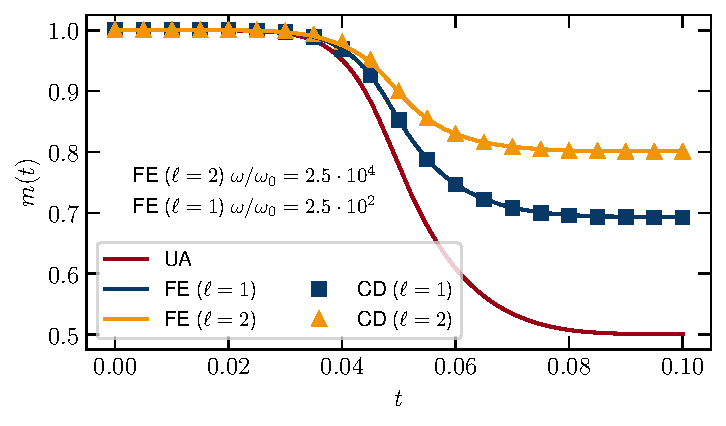
\includegraphics[height=7cm]{img/demo-plot.pdf}
    \caption{Simple example of plot saved in PDF and imported in the document. This ensures correctly vectorized images.}
    \label{fig:demo-plot}
\end{figure}


\lipsum[1-5]






\section{Drawing with tikz}

When you get skilled, you might want to create drawings in \texttt{tikz}, like in Figure~\ref{fig:demo-max-cut}.
You can make equations with drawings,
% note: this is an equation with drawings\
\input{img/drawings/demo-eq-tikz}
or tables with drawings, like in Table~\ref{tab:demo-draw}... 

\lipsum[1-2]



\begin{figure}
    \centering
    \input{img/drawings/demo-maxcut}
    \caption{An example of Maximum Cut problem. The dashed line cuts the seven edges that are highlighted in red. Consequently, the vertices are marked with different colors to indicate their belonging to partition $U$ or $\bar{U}$.}
    \label{fig:demo-max-cut}
\end{figure}



\begin{table}
\centering
\begin{tblr}{colspec={Q[c,h]cccc},stretch=0,rowsep=6pt}
\hline
spin indexing&N&label&sign of $J_k$&$\theta$\\\hline
\SetCell[r=3]{m} \scalebox{0.6}{\input{img/drawings/demo-lhz6}} & \SetCell[r=3]{m} 6 
    & LHZ6E & $[+,+,-,-,+,-]$ &0.0 \\\hline
&   & \textbf{LHZ6M} & $[-,-,-,+,-,+]$ & 0.3\\\hline
&   & LHZ6H & $[+,+,+,-,-,+]$ & 0.55\\\hline
\hspace{-3mm}\scalebox{0.6}{\input{img/drawings/demo-lhz10}} & 10 & LHZ10&\makecell{$[-,-,-,-,+$\\$\;\;+,+,-,-,-]$}&0.3\\
\hline
\end{tblr}
    \caption{\label{tab:demo-draw} Selected instances of LHZ models that are considered in the following analysis. The constraints are fixed to $C_l=-2$ and the magnitude of the local fields to $|J_k|=1$. The signs of $J_k$ that fully determine the instance are reported in the table, along with the label of the instance and its ``hardness'' $\theta$. The reference study case is LHZ6M.}
\end{table}

\section{Special boxes}

The template offers special environments for important text and comments...
\begin{info}
... like this one, \texttt{info}. Other special environments are \texttt{warning} and \texttt{example}, which differ from this only by the icon on the top left of the delimited area.
\end{info}
You can define your own custom environment via an \texttt{mdfdefinestyle}.
Have a look at \textit{template/extras.tex} for a reference.

\subsection{Code snippets}

The template integrates \texttt{listings} as the default environment for code snippets. You can define your own style in \textit{template/extras.tex}.

\begin{lstlisting}[language=Python]
def half(n: int): # comment
    return "the half is" + str(n//2)
\end{lstlisting}


\section{PDF/A compliance}

The University submission system requires the final manuscript to be provided as a PDF/A compliant document.
For this reason, this template enforces the \textbf{PDF/A-2b} standard at compilation time through the \verb|pdfx| package.

To verify compliance of the generated PDF, you may use an online validation service such as
\href{https://www.pdfforge.org/online/en/validate-pdfa}{pdfforge PDF/A validator}.\\

\noindent
\textbf{Compiler compatibility.}
As of 2026, some incompatibilities have been observed between PDF/A generation and the \verb|pdfLaTeX| compiler when using the Palatino text font package \verb|newpxtext| adopted by this template.
These issues may result in PDF/A validation errors related to embedded font consistency.

For this reason, the recommended compiler for this template is \textbf{LuaLaTeX}, which provides full compatibility with the default font configuration and generally produces valid PDF/A output without requiring further modifications.

If LuaLaTeX is not available, the following alternatives may be considered:

\begin{itemize}
    \item \textbf{Use pdfLaTeX with \texttt{mathpazo}.}  
    This requires editing the template class file and replacing \verb|newpxtext| with \verb|mathpazo| (already included as a commented alternative). This configuration is PDF/A compliant, although it produces slightly different text and mathematical typography.

    \item \textbf{Post-process the generated PDF.}  
    If your document relies on packages or graphical features that interfere with PDF/A compliance (for instance transparency effects or unsupported font configurations), you may generate a standard PDF and convert it afterward using an external PDF/A conversion service such as
    \href{https://www.pdfforge.org/online/en/pdf-to-pdfa}{pdfforge PDF/A converter}.
\end{itemize}

The available PDF/A workflows are summarized in Table~\ref{tab:pdfa}.

\begin{table}[h!]
\small
\centering
\def\arraystretch{1.4}
\begin{tabular}{c|p{2.8cm}|c|c}\hline
\textbf{Option} & \textbf{Font package} & \textbf{pdfLaTeX} & \textbf{LuaLaTeX (recommended)} \\
\hline\hline
1 & \verb|newpxtext| 
& Known PDF/A compatibility issues 
& Works out of the box \\
\hline
2 & \verb|mathpazo| 
& Works out of the box 
& Works out of the box \\
\hline
3 & \multicolumn{3}{c}{Use external conversion to PDF/A on compiled document.}\\
\hline
\end{tabular}
\caption{\label{tab:pdfa}Available workflows for PDF/A-compliant document generation.}
\end{table}

    % NOTE: I suggest to create a file for each chapter, like the previous \input{}.


    % II -----------------------
    \part{\label{prt:filler}Filler part}
    
    %!TEX root = ../main.tex

\chapter{Filling with text}\label{ch:filling}

\lipsum[1-4]

\section{Lipsum}
\lipsum[5-7]

\section{is}
\lipsum[8-10]

\section{useful}
\lipsum[11-14]



\chapter{Filling with more text: two-line chapter title}\label{ch:filling-more}

\lipsum[15-16]

\section{UniPd is the best}
\lipsum[19-21]

\section{Latex}
\lipsum[28-30]

\subsection{Latex again}
\lipsum[30-31]

\subsection{Latex for good}
\lipsum[32-33]


    % conclusion ---------------
    \bookmarksetup{startatroot}
    %!TEX root = ../main.tex

\addtocontents{toc}{\protect\vskip1em}
\chapter*{Conclusions}\label{ch:conclusions}
\markboth{Conclusions}{}
\addcontentsline{toc}{chapter}{Conclusions} 
%  NOTE: Introduction and Conclusions are special chapters: they are not
% marked by a section number, so we need to add it manually to the
% ToC, as done above.
% The line above \chapter* serves to create a space between the previous 
% chapters/parts and the conclusion. Feel free to remove it if not needed.

\lipsum[1-10]


    % appendices ---------------
    \begin{appendices}
        %!TEX root = ../main.tex

\chapter{An amazing appendix}\label{ax:demo}

\lipsum[1-10]

    \end{appendices}

    % glossary, bibliography, acknowledges
    \backmatter
\end{document}%!TEX TS-program = pdflatex
%!TEX encoding = UTF-8 Unicode

\documentclass{unipd-thesis-modern} % src: https://github.com/baronefr/unipd-thesis-modern
%  print layout: two-sided with binding on the left


% I recommend to validate/convert the PDF/A file with the following tool:
% https://www.pdfforge.org/online/en/validate-pdfa


% additional packages
\usepackage{lipsum} % for DEMO only

%% (optional) to add a draft watermark, uncomment the following:
%\usepackage[color={[gray]{0.85}}]{draftwatermark}
%% NOTE: high values -> less visible

% ToC customization
\setlength{\cftbeforechapskip}{7pt} % there are more variables like this set in the template file
\setcounter{tocdepth}{4} % ToC depth


% titles
\title{A modern template for a thesis at\\ the University of Padova}
\thesisHeader{Department of Physics and Astronomy ``G. Galilei''\\PhD Thesis in Physics}
\academicYear{2026/2027}

% student
\author{Student Name Surname}
\studentId{1234567}

% supervisor(s)Zürich
\advisor{Prof. Manuel Rolo}{INFN Turin} % (mandatory)
\coadvisor{Dr. Alberto Tibaldi}{Politechnico di Torino} % (optional, comment to remove)
\otheradvisor{Prof. Paolino Paperino}{University of Padova} % (optional, comment to remove)
% ^ NOTE: you can use optional arg to customize the label "Internal Supervisor"
%   example:   \otheradvisor[The best supervisor!]{Prof. Paolino Paperino}{University of Padua}




% add notes at the bottom of the second page (optional)
\secondpage{\mbox{}
\vfill

{\small\onehalfspacing
\begin{center}

\noindent\rule{\textwidth}{1pt} % ----------

    \LaTeX~document compiled on \today.

\noindent\rule{\textwidth}{.2pt} % ----------

    \textbf{Additional resources}
    
    This template allows you to put some text in the second cover page.\\ 
    The text can be modified in \textit{docs/secondcover.tex}.\\
    I suggest you take this space to refer to any software repository linked to your work,\\ such as the following:\\

    \prettygitlink{sami12398987/Unipd-thesis-template}
\end{center}
} % ----------}

% dedication (comment line to remove)
\dedication{\textit{To my parents\\and friends}}


% define custom symbols and shortcuts (optional)
%!TEX root = ./main.tex

% please use this file to define custom symbols and commands

\newtheorem{prop}{Proposition}
\newtheorem{theorem}{Theorem}

\newcommand{\myvec}[1]{\underline{#1}}

\newcommand{\hamCD}{\mathcal{H}_{\mathrm{CD}}}
\newcommand{\hamFE}{\mathcal{H}_{\mathrm{FE}}}
\newcommand{\hamUA}{\mathcal{H}_{\mathrm{UA}}}

\newcommand{\equalexpl}[1]{%
  \underset{\substack{\uparrow\\\mathrlap{\text{\hspace{-1em}#1}}}}{=}}


% bibliography file
\addbibresource{refs.bib}

%% SUGGESTION: to print only the cover page with larger fonts and without watermark, uncomment the following:
%\begin{document}
%    \makecover
%\end{document}


\begin{document}
    % cover, ToC, abstract
    \frontmatter

    % main content
    \mainmatter

    % introduction -------------
    %!TEX root = ../main.tex

\chapter*{Introduction}\label{ch:introduction}
\markboth{Introduction}{}
\addcontentsline{toc}{chapter}{Introduction} 
% NOTE: Introduction and Conclusions are special chapters: they are not
%       marked by a section number, so we need to add it manually to the
%       ToC, as done above.

\lipsum[1-7]

    \glsresetall  % reset gls after introduction (suggested, but optional)


    % I  -----------------------
    \part{\label{prt:demo}Demo of the template features} % NOTE: dividing in parts is optional

    %!TEX root = ../main.tex

\chapter{Basic template features}\label{ch:feats}

I assume you already know how to use \LaTeX, so I won't write a lot.
Some \emph{words} are more important than others, so you might want to \emph{emphasize} them with the \verb|\emph| command.
On the other hand, you might wanna tell more about something without taking up a lot of space in the main text.
That's when you use footnotes\footnote{Just use the command \texttt{footnote}.}.

In a good scientific text, it is crucial to cite other people's work. If you say something important, make sure to \verb|\cite| it soon afterward \cite{10.1088/1367-2630/ad313e}. By the way, Ref.~\cite{10.1088/1367-2630/ad313e} is not saying anything useful for this purpose, so don't look at it. The bibliography entries are located in \texttt{refs.bib}.




\section{Math}

An equation might look like this $\mathcal{H}(\lambda) = A(t)\mathcal{H}_{A} + B(t)\mathcal{H}_{B}$, if inline. 
Otherwise, you might take more space:
\begin{equation*}
    \mathcal{H}(\lambda) = A(t)\mathcal{H}_{A} + B(t)\mathcal{H}_{B} + C(t)\mathcal{H}_{C} + ...
\end{equation*}

I will put here more math stuff with equations, just to make my point. Let $\ket{\psi(t)}$ be a quantum state that evolves in the time interval $[0,\tau]$. Its dynamics are described by the time-dependent Schrödinger equation.
$$i\ket{\dot\psi(t)} = \mathcal{H}(t)\ket{\psi(t)}$$
We use from now on the natural units $\hbar=1$. Let us introduce the basis of instantaneous eigenstates $\ket{n(t)}$ with eigenvalues $\epsilon_n(t)$:
\begin{equation}
    \label{eq:adth-eigenvalue}
    \mathcal{H}(t)\ket{n(t)} = \epsilon_n(t) \ket{n(t)}
\end{equation}
Since $\{\ket{n(t)}\}$ is a complete orthonormal set, $\ket{\psi(t)}$ can be expressed as a linear combination in that basis:
\begin{equation}
    \ket{\psi(t)} = \sum_n c_n(t) e^{i\theta_n(t)} \ket{n(t)}
\end{equation}
We have explicitly factorized the phase $\theta_n(t)=\int_0^t \epsilon_n(t')dt'$ from $c_n(t)$. This choice will be convenient in the following calculations, but it can be intuitively motivated straight away. 
It is known that an eigenstate picks up a phase $e^{-i\epsilon_n}$ when it evolves under a constant Hamiltonian. The $\theta_n(t)$ is a generalization of the picked-up phase, obtained by integrating it throughout the time interval in which the Hamiltonian evolves. It is known as the Berry phase.\\


To show the use of \verb|\underbrace{}|, we now write the Schrödinger equation in a rotating frame:
\begin{align}
    i\frac{d\ket{\tilde{\psi}}}{dt} &= i\left( \frac{dU^\dag}{dt}\ket{\psi} + U^\dag \frac{d\ket{\psi}}{dt} \right) = \nonumber\\
    &= i\dot\lambda \partial_\lambda U^\dag \cdot U\ket{\tilde{\psi}} + U^\dag\mathcal{H}\cdot U\ket{\tilde{\psi}} =\nonumber\\
    & \equiv \underbrace{\left( \tilde{\mathcal{H}} - \dot\lambda \tilde{\mathcal{A}}_\lambda \right)}_{\mathcal{H}_{rot}}\ket{\tilde{\psi}} \label{eq:schr-movingframe}
\end{align}

Just a suggestion: define recurrent symbols in \texttt{custom-symbols.tex}. For instance, typing \verb|\hamCD| to print $\hamCD$ is way more compact than typing
\begin{center}
    \verb|\mathcal{H}_{\mathrm{CD}}|
\end{center}
all the time...





\subsection{Theorem support}

You might input some theorem!

\begin{theorem}
Suppose that the spectrum of $\mathcal{H}(\lambda)$ has the ground state eigenvalue separated by a gap $\Delta(\lambda)=\epsilon_1(\lambda)-\epsilon_0(\lambda)\ >0$ from the rest of the spectrum, and that $\mathcal{H}$ is twice continuously differentiable. Assume that $\mathcal{H}$, $\partial_\lambda\mathcal{H}$ and $\partial^2_\lambda\mathcal{H}$ are bounded operators (an assumption that is always fulfilled in finite-dimensional spaces). Then
\begin{equation}
    \tau \gg \max\left(
        \max_\lambda \frac{\|\partial_\lambda\mathcal{H}(\lambda)\|}{\Delta^2(\lambda)},
        \max_\lambda \frac{\|\partial^2_\lambda\mathcal{H}(\lambda)\|}{\Delta^2(\lambda)}, 
        \max_\lambda \frac{\|\partial_\lambda\mathcal{H}(\lambda)\|^2}{\Delta^3(\lambda)}
    \right) .
\end{equation}
\end{theorem}








\section{Glossary}

In \texttt{docs/glossary.tex}, one might introduce acronyms that are printed in the table at the end of the document. The syntax is simple:

\begin{center}
    \verb|\newacronym{acronym-label}{EAT}{Extended Acronym Text}|
\end{center}

To reference the acronym, use the command \verb|\gls|. 
In the previous example, the command \verb|\gls{acronym-label}| will print:
\begin{itemize}
    \item \gls{acronym-label}, if the acronym has not been used before.
    \item \gls{acronym-label}, if the acronym has already been used in the text.
    \item Here, \gls{acronym-label} has been called for the third time!
\end{itemize}

It is possible to reset the counter for all the acronyms with \verb|\glsresetall|, or to reset the counter for a specific acronym with \verb|\glsreset{acronym-label}|.

\section{Colors}\label{sec:color}

The template is defined around color identifiers. \texttt{mainColor} is set to the classic red color of the UniPD color palette.
By default, the color of the rectangle in the Chapter headlines and the color of the box in the Part page are inherited from the main color,
\begin{lstlisting}[language={[latex]TeX}]
\colorlet{chapterColor}{mainColor}
\colorlet{partBoxColor}{mainColor}
\end{lstlisting}
which you can change by redefining the color inside the \texttt{.cls} template:
\begin{lstlisting}[language={[latex]TeX}]
\definecolor{chapterColor}{RGB}{255, 187, 0}
\end{lstlisting}


\section{References and floating objects}

Using the \verb|\ref| command, you might reference labeled objects.
Chapter~\ref{ch:feats} is the only useful chapter of this template.
All the others, in Part~\ref{prt:filler}, are just filled with \texttt{lipsum} text.
The appendices are referenced with letters: for instance Appendix~\ref{ax:demo}.\\

When referencing equations, it is recommended to use \verb|\eqref| instead. 
For instance, Eq.~\eqref{eq:adth-eigenvalue} is clearly understood by any physics undergraduate!\\

Tables in \LaTeX are quite nice! Take a look at Table~\ref{tab:demo}.\\

\begin{table}[h]
\centering
\begin{tabular}{c|c|cc|cc}
    &\multirow{2}{*}{UA}&\multicolumn{2}{c|}{CD}&\multicolumn{2}{c}{FE}\\
    &&$\ell=1$&$\ell=2$&$\ell=1$&$\ell=2$\\\hline
    $f(\tau) \;[10^{-2}]$&1.5793&7.4970&17.039&7.5554&17.162\\
    $m(\tau)$&0.50107&0.69264&0.80038&0.69354&0.80143\\
    \hline
\end{tabular}
\caption{\label{tab:demo}Fidelity and energy merit resulting from an annealing simulation.}
\end{table}



Another kind of floating object are, of course, figures! To keep it simple, look at Figure~\ref{fig:demo}.\\

\begin{figure}
    \centering
    \includegraphics[height=6cm]{example-image-a}
    \caption{Simple example of floating image demo.}
    \label{fig:demo}
\end{figure}


As for plots, I recommend you save them in PDF format (Figure~\ref{fig:demo-plot}).

\begin{figure}
    \centering
    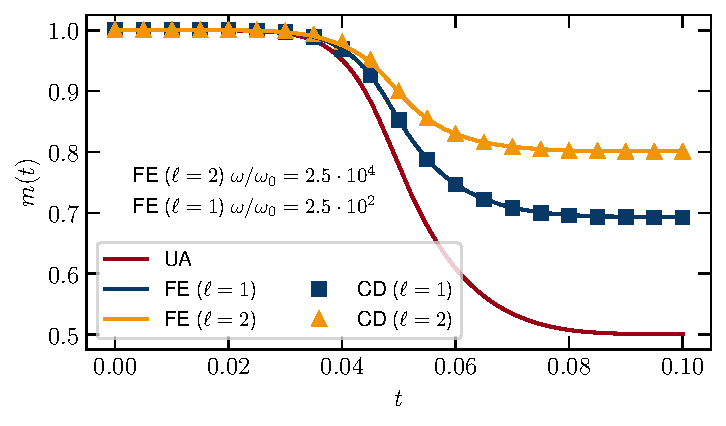
\includegraphics[height=7cm]{img/demo-plot.pdf}
    \caption{Simple example of plot saved in PDF and imported in the document. This ensures correctly vectorized images.}
    \label{fig:demo-plot}
\end{figure}


\lipsum[1-5]






\section{Drawing with tikz}

When you get skilled, you might want to create drawings in \texttt{tikz}, like in Figure~\ref{fig:demo-max-cut}.
You can make equations with drawings,
% note: this is an equation with drawings\
\input{img/drawings/demo-eq-tikz}
or tables with drawings, like in Table~\ref{tab:demo-draw}... 

\lipsum[1-2]



\begin{figure}
    \centering
    \input{img/drawings/demo-maxcut}
    \caption{An example of Maximum Cut problem. The dashed line cuts the seven edges that are highlighted in red. Consequently, the vertices are marked with different colors to indicate their belonging to partition $U$ or $\bar{U}$.}
    \label{fig:demo-max-cut}
\end{figure}



\begin{table}
\centering
\begin{tblr}{colspec={Q[c,h]cccc},stretch=0,rowsep=6pt}
\hline
spin indexing&N&label&sign of $J_k$&$\theta$\\\hline
\SetCell[r=3]{m} \scalebox{0.6}{\input{img/drawings/demo-lhz6}} & \SetCell[r=3]{m} 6 
    & LHZ6E & $[+,+,-,-,+,-]$ &0.0 \\\hline
&   & \textbf{LHZ6M} & $[-,-,-,+,-,+]$ & 0.3\\\hline
&   & LHZ6H & $[+,+,+,-,-,+]$ & 0.55\\\hline
\hspace{-3mm}\scalebox{0.6}{\input{img/drawings/demo-lhz10}} & 10 & LHZ10&\makecell{$[-,-,-,-,+$\\$\;\;+,+,-,-,-]$}&0.3\\
\hline
\end{tblr}
    \caption{\label{tab:demo-draw} Selected instances of LHZ models that are considered in the following analysis. The constraints are fixed to $C_l=-2$ and the magnitude of the local fields to $|J_k|=1$. The signs of $J_k$ that fully determine the instance are reported in the table, along with the label of the instance and its ``hardness'' $\theta$. The reference study case is LHZ6M.}
\end{table}

\section{Special boxes}

The template offers special environments for important text and comments...
\begin{info}
... like this one, \texttt{info}. Other special environments are \texttt{warning} and \texttt{example}, which differ from this only by the icon on the top left of the delimited area.
\end{info}
You can define your own custom environment via an \texttt{mdfdefinestyle}.
Have a look at \textit{template/extras.tex} for a reference.

\subsection{Code snippets}

The template integrates \texttt{listings} as the default environment for code snippets. You can define your own style in \textit{template/extras.tex}.

\begin{lstlisting}[language=Python]
def half(n: int): # comment
    return "the half is" + str(n//2)
\end{lstlisting}


\section{PDF/A compliance}

The University submission system requires the final manuscript to be provided as a PDF/A compliant document.
For this reason, this template enforces the \textbf{PDF/A-2b} standard at compilation time through the \verb|pdfx| package.

To verify compliance of the generated PDF, you may use an online validation service such as
\href{https://www.pdfforge.org/online/en/validate-pdfa}{pdfforge PDF/A validator}.\\

\noindent
\textbf{Compiler compatibility.}
As of 2026, some incompatibilities have been observed between PDF/A generation and the \verb|pdfLaTeX| compiler when using the Palatino text font package \verb|newpxtext| adopted by this template.
These issues may result in PDF/A validation errors related to embedded font consistency.

For this reason, the recommended compiler for this template is \textbf{LuaLaTeX}, which provides full compatibility with the default font configuration and generally produces valid PDF/A output without requiring further modifications.

If LuaLaTeX is not available, the following alternatives may be considered:

\begin{itemize}
    \item \textbf{Use pdfLaTeX with \texttt{mathpazo}.}  
    This requires editing the template class file and replacing \verb|newpxtext| with \verb|mathpazo| (already included as a commented alternative). This configuration is PDF/A compliant, although it produces slightly different text and mathematical typography.

    \item \textbf{Post-process the generated PDF.}  
    If your document relies on packages or graphical features that interfere with PDF/A compliance (for instance transparency effects or unsupported font configurations), you may generate a standard PDF and convert it afterward using an external PDF/A conversion service such as
    \href{https://www.pdfforge.org/online/en/pdf-to-pdfa}{pdfforge PDF/A converter}.
\end{itemize}

The available PDF/A workflows are summarized in Table~\ref{tab:pdfa}.

\begin{table}[h!]
\small
\centering
\def\arraystretch{1.4}
\begin{tabular}{c|p{2.8cm}|c|c}\hline
\textbf{Option} & \textbf{Font package} & \textbf{pdfLaTeX} & \textbf{LuaLaTeX (recommended)} \\
\hline\hline
1 & \verb|newpxtext| 
& Known PDF/A compatibility issues 
& Works out of the box \\
\hline
2 & \verb|mathpazo| 
& Works out of the box 
& Works out of the box \\
\hline
3 & \multicolumn{3}{c}{Use external conversion to PDF/A on compiled document.}\\
\hline
\end{tabular}
\caption{\label{tab:pdfa}Available workflows for PDF/A-compliant document generation.}
\end{table}

    % NOTE: I suggest to create a file for each chapter, like the previous \input{}.


    % II -----------------------
    \part{\label{prt:filler}Filler part}
    
    %!TEX root = ../main.tex

\chapter{Filling with text}\label{ch:filling}

\lipsum[1-4]

\section{Lipsum}
\lipsum[5-7]

\section{is}
\lipsum[8-10]

\section{useful}
\lipsum[11-14]



\chapter{Filling with more text: two-line chapter title}\label{ch:filling-more}

\lipsum[15-16]

\section{UniPd is the best}
\lipsum[19-21]

\section{Latex}
\lipsum[28-30]

\subsection{Latex again}
\lipsum[30-31]

\subsection{Latex for good}
\lipsum[32-33]


    % conclusion ---------------
    \bookmarksetup{startatroot}
    %!TEX root = ../main.tex

\addtocontents{toc}{\protect\vskip1em}
\chapter*{Conclusions}\label{ch:conclusions}
\markboth{Conclusions}{}
\addcontentsline{toc}{chapter}{Conclusions} 
%  NOTE: Introduction and Conclusions are special chapters: they are not
% marked by a section number, so we need to add it manually to the
% ToC, as done above.
% The line above \chapter* serves to create a space between the previous 
% chapters/parts and the conclusion. Feel free to remove it if not needed.

\lipsum[1-10]


    % appendices ---------------
    \begin{appendices}
        %!TEX root = ../main.tex

\chapter{An amazing appendix}\label{ax:demo}

\lipsum[1-10]

    \end{appendices}

    % glossary, bibliography, acknowledges
    \backmatter
\end{document}
